%%%%%%%%%%%%%%%%%%%%%%%%%%%%%%%%%%%%%%%%%%%%%%%%%%%%%%%%%%%%%%%%%%%%%%%%%%%%%%%%
% Template for USENIX papers.
%
% History:
%
% - TEMPLATE for Usenix papers, specifically to meet requirements of
%   USENIX '05. originally a template for producing IEEE-format
%   articles using LaTeX. written by Matthew Ward, CS Department,
%   Worcester Polytechnic Institute. adapted by David Beazley for his
%   excellent SWIG paper in Proceedings, Tcl 96. turned into a
%   smartass generic template by De Clarke, with thanks to both the
%   above pioneers. Use at your own risk. Complaints to /dev/null.
%   Make it two column with no page numbering, default is 10 point.
%
% - Munged by Fred Douglis <douglis@research.att.com> 10/97 to
%   separate the .sty file from the LaTeX source template, so that
%   people can more easily include the .sty file into an existing
%   document. Also changed to more closely follow the style guidelines
%   as represented by the Word sample file.
%
% - Note that since 2010, USENIX does not require endnotes. If you
%   want foot of page notes, don't include the endnotes package in the
%   usepackage command, below.
% - This version uses the latex2e styles, not the very ancient 2.09
%   stuff.
%
% - Updated July 2018: Text block size changed from 6.5" to 7"
%
% - Updated Dec 2018 for ATC'19:
%
%   * Revised text to pass HotCRP's auto-formatting check, with
%     hotcrp.settings.submission_form.body_font_size=10pt, and
%     hotcrp.settings.submission_form.line_height=12pt
%
%   * Switched from \endnote-s to \footnote-s to match Usenix's policy.
%
%   * \section* => \begin{abstract} ... \end{abstract}
%
%   * Make template self-contained in terms of bibtex entires, to allow
%     this file to be compiled. (And changing refs style to 'plain'.)
%
%   * Make template self-contained in terms of figures, to
%     allow this file to be compiled. 
%
%   * Added packages for hyperref, embedding fonts, and improving
%     appearance.
%   
%   * Removed outdated text.
%
%%%%%%%%%%%%%%%%%%%%%%%%%%%%%%%%%%%%%%%%%%%%%%%%%%%%%%%%%%%%%%%%%%%%%%%%%%%%%%%%

\documentclass[letterpaper,twocolumn,10pt]{article}
\usepackage{usenix-2020-09}

% to be able to draw some self-contained figs
\usepackage{tikz}
\usepackage{amsmath}

% inlined bib file
\usepackage{filecontents}

%-------------------------------------------------------------------------------
\begin{filecontents}{\jobname.bib}
%-------------------------------------------------------------------------------
@Book{arpachiDusseau18:osbook,
  author =       {Arpaci-Dusseau, Remzi H. and Arpaci-Dusseau Andrea C.},
  title =        {Operating Systems: Three Easy Pieces},
  publisher =    {Arpaci-Dusseau Books, LLC},
  year =         2015,
  edition =      {1.00},
  note =         {\url{http://pages.cs.wisc.edu/~remzi/OSTEP/}}
}
@InProceedings{waldspurger02,
  author =       {Waldspurger, Carl A.},
  title =        {Memory resource management in {VMware ESX} server},
  booktitle =    {USENIX Symposium on Operating System Design and
                  Implementation (OSDI)},
  year =         2002,
  pages =        {181--194},
  note =         {\url{https://www.usenix.org/legacy/event/osdi02/tech/waldspurger/waldspurger.pdf}}}
\end{filecontents}

%-------------------------------------------------------------------------------
\begin{document}
%-------------------------------------------------------------------------------

%don't want date printed
\date{}

% make title bold and 14 pt font (Latex default is non-bold, 16 pt)
\title{\Large \bf Research Proposal: \\Pruning Techniques for the Quanto Quantum Curcuit Optimizer}

%for single author (just remove % characters)
\author{
{\rm Max von Storch}\\
Technische Universität München
\and
{\rm Johannes Schielein}\\
Technische Universität München
% copy the following lines to add more authors
% \and
% {\rm Name}\\
%Name Institution
} % end author

\maketitle

%-------------------------------------------------------------------------------
\begin{abstract}
%-------------------------------------------------------------------------------
This report is about Quanto, a quantum circuit optimizers with uses automated circuit identity generation, and our approach to optimize
it by pruning the space of possible circuits.   
\end{abstract}


%-------------------------------------------------------------------------------
\section{Part A: Paper Summary}
%-------------------------------------------------------------------------------

\subsection{Context of the work (``Why?'')}

Quantum compilers are used to optimize circuits in an effort to reduce execution time, the noise that naturally arises in quantum computations, or both. Generally, the larger the circuit depth, the noisier the computation, leading to more errors in the results. As quantum programs must be executed many times to obtain an accurate picture of their results, reducing the depth of a quantum circuit not only makes a quantum program faster but also reduces the potential for noise and decreases the number of program evaluations required. By optimizing the circuit, quantum compilers enhance the overall efficiency and reliability of quantum computations.
\\\\
Existing quantum compilers focus on mapping logical quantum circuits to quantum devices and their native quantum gates. This involves translating source gates to target gates and adapting the circuit to hardware constraints like qubit connectivity. Typically, only simple circuit identities are used during this process, which overlooks the potential for more complex optimizations.
\\\\
Compilers developed by hardware vendors, such as IBM and Google, primarily address the translation and hardware adaptation aspects but pay less attention to optimizing the logical circuit itself by finding comprehensive circuit identities. While circuit identities have been manually identified and automatically generated for single-qubit gates, no current system automatically finds identities for full gate sets or optimizes quantum circuits based on these identities.
\\\\
For example, the Verified Optimizer for Quantum Circuits (voqc) applies a limited set of optimization rules: not propagation, Hadamard reduction, single-qubit gate cancellation, two-qubit gate cancellation, and rotation merging, in a specific sequence. These limited rules restrict the potential for discovering more effective optimizations.
\subsection{Contributions of the work (``How?'')}

Quanto automatically generates circuit identities for full gate sets and operates trough two main phases: (1) Identity generation (2) circuit optimization (Fig. \ref{fig:quanto_system_design}).
\\\\
In the identity generation phase, all possible circuit identities are generated for a specified depth and number of qubits. These identities are stored in a hash table, using the hash of their unitary matrices as keys, enabling quick lookup by the optimizer.
\\\\
In the circuit optimization phase, the input quantum circuit is divided into smaller sub-circuits, or tiles. The optimizer looks up the fingerprint of each tile in the hash table to find equivalent circuit identities. These identities replace the original sub-circuits, iteratively optimizing the circuit until the most efficient version is achieved.

\subsubsection{Circuit Identity Generator}
\textbf{Step 1: Represent the quantum circuit as a grid.}
The algorithm starts by representing a quantum circuit as a grid. The number of rows $d$ represents the layers in the quantum circuit, also known as the circuit depth, and the number of columns $n$ represents the number of qubits. If no gate is present at a particular position, the identity gate is placed there (Fig. \ref{fig:quanto_example_grid}).
\\\\
\textbf{Step 2: Generation of all possible circuits for $d = 1$.}
If the gate set contains two-qubit gates, these gates are split into the first and second qubit they operates on (Fig. \ref{}).
\\\\
\textbf{Step 3: Generation of all possible circuits for $d > 1$.}
All subsequent circuits are generated by iteratively appending circuits of depth one ($d=1$) to each previously generated circuit. This process effectively generates the "cross-product" of circuits with the current depth and circuits of depth one (Fig. \ref{}).
\\\\
\textbf{Step 4: Calculation of unitary matrices and hash values.}
For each generated circuit, the algorithm calculates the unitary matrix. To avoid expensive computations repeatedly, it computes a hash value (fingerprint) for each circuit based on its unitary matrix. This fingerprint uniquely identifies the circuit's functionality.
\\\\
\textbf{Step 6: Create fingerprint database.}
The fingerprints are stored in a hash table, with the circuit structure as the key and the fingerprint as the value (Fig. \ref{}). This enables quick look-up of a circuit’s fingerprint during the optimization phase without recalculating the unitary matrix.
\\\\
\textbf{Step 7: Create identity database.}
Circuits with identical fingerprints are stored together, forming equivalence classes of circuits (Fig. \ref{}). Each entry in this hash table represents a set of circuits that perform the same quantum operation but may have different structures.
\\\\

\subsubsection{Circuit Optimizer}
\textbf{Step 1: Generate tiles.}
The circuit is divided into sub-circuits, referred to as tiles. Tiles have uniform dimensions, with the tile width $j$ representing the maximum depth $d$ of the circuit identities, and the tile length $i$ representing the maximum number of qubits $n$. The number of possible $i \times j$ tiles for an $n \times d$ circuit is $(n-i+1) \cdot (d-j+1)$.
\\\\
\textbf{Step 2: Check tile validity.}
A tile is invalid and therefore discarded if it contains a two-qubit gate that is not placed at the boundaries of the tile and is cut off by the tile (Fig. \ref{}).
\\\\
\textbf{Step 3: Tile lookup.}
If a tile contains a two-qubit gate, that has been cut off only at the boundaries of the tile, the cut off gate has to be replaced by an Identity gate, so that there will be a match in the circuit identity database (Fig. \ref{}). Now the fingerprint is retrieved from the fingerprint database, without having to calculate the unitary matrix. 
\\\\
\textbf{Step 4: Apply substitution.}
For each tile, the corresponding circuit identities are iterated and evaluated by the customizable cost function. In the paper, the cost function optimizes the circuit according to the depth $d$ of the circuit. 
\\\\
\textbf{Step 5: Apply substitution to the circuit.}
The optimizer applies the substitution to the quantum circuit (Fig. \ref{}). If a $CX$ gate was replaced by an identity gate in the tile, the identity gate in the actual circuit must be replaced by a $CX$ gate during the substitution (Fig. \ref{}). 
\\\\
\textbf{Step 6: Repeat process.}
Repeat steps 1-6 for a fixed number of times.

\subsection{Evaluation}
\subsubsection{Generation of novel identities}
Quanto is capable of automatically discovering identities known from previous work and generating novel identities, especially for two-qubit gates. By leveraging its automated circuit identity generation capabilities, Quanto can find optimizations that are not identified by other compilers. For example, in evaluating the IBM Qiskit compiler, Quanto generated novel circuit identities that the Qiskit compiler could not find. This capability is particularly useful for quantum hardware with non-standard native gate sets.
\subsubsection{Challenge of scalability}
One of the main challenges faced by Quanto is scalability. The vast space of potential circuit identities and the high computational resources required to generate these identities present significant hurdles. As the number of qubits $n$ and the circuit depth $d$ increase, the number of possible circuits grows exponentially, making it computationally expensive to handle larger circuits. Moreover, many useless identities are stored in the database, contributing to redundancy and inefficiency. Additionally, the tiling approach may limit the ability to find large-scale identities, as it is constrained by the maximum depth of circuit identities it can handle.

%-------------------------------------------------------------------------------
\section{Part B: Research proposal (2 pages)}
%-------------------------------------------------------------------------------

\subsection{Context of your research (``Why?'')}
\begin{itemize}
  \item \textbf{What is the problem?}
  \item \textbf{Why is it important or interesting?}
  \item \textbf{Why is it difficult? Or what are the challenges?}
\end{itemize}

\subsection{Approach of your research work (``How?'')}
\begin{itemize}
  \item \textbf{What is the proposed solution? How does it work?}
  \item \textbf{What are the key insights?}
  \item \textbf{Or what are the novel aspects?}
\end{itemize}

%-------------------------------------------------------------------------------
\section{Footnotes, Verbatim, and Citations}
%-------------------------------------------------------------------------------

Footnotes should be places after punctuation characters, without any
spaces between said characters and footnotes, like so.%
\footnote{Remember that USENIX format stopped using endnotes and is
  now using regular footnotes.} And some embedded literal code may
look as follows.

\begin{verbatim}
int main(int argc, char *argv[]) 
{
    return 0;
}
\end{verbatim}

Now we're going to cite somebody. Watch for the cite tag. Here it
comes. Arpachi-Dusseau and Arpachi-Dusseau co-authored an excellent OS
book, which is also really funny~\cite{arpachiDusseau18:osbook}, and
Waldspurger got into the SIGOPS hall-of-fame due to his seminal paper
about resource management in the ESX hypervisor~\cite{waldspurger02}.

The tilde character (\~{}) in the tex source means a non-breaking
space. This way, your reference will always be attached to the word
that preceded it, instead of going to the next line.

And the 'cite' package sorts your citations by their numerical order
of the corresponding references at the end of the paper, ridding you
from the need to notice that, e.g, ``Waldspurger'' appears after
``Arpachi-Dusseau'' when sorting references
alphabetically~\cite{waldspurger02,arpachiDusseau18:osbook}. 

It'd be nice and thoughtful of you to include a suitable link in each
and every bibtex entry that you use in your submission, to allow
reviewers (and other readers) to easily get to the cited work, as is
done in all entries found in the References section of this document.

Now we're going take a look at Section~\ref{sec:figs}, but not before
observing that refs to sections and citations and such are colored and
clickable in the PDF because of the packages we've included.

%-------------------------------------------------------------------------------
\section{Floating Figures and Lists}
\label{sec:figs}
%-------------------------------------------------------------------------------


%---------------------------
\begin{figure}
\begin{center}
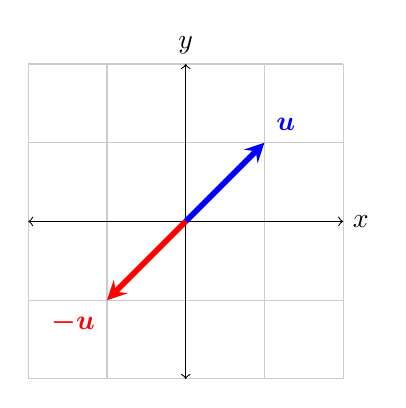
\begin{tikzpicture}
  \draw[thin,gray!40] (-2,-2) grid (2,2);
  \draw[<->] (-2,0)--(2,0) node[right]{$x$};
  \draw[<->] (0,-2)--(0,2) node[above]{$y$};
  \draw[line width=2pt,blue,-stealth](0,0)--(1,1)
        node[anchor=south west]{$\boldsymbol{u}$};
  \draw[line width=2pt,red,-stealth](0,0)--(-1,-1)
        node[anchor=north east]{$\boldsymbol{-u}$};
\end{tikzpicture}
\end{center}
\caption{\label{fig:vectors} Text size inside figure should be as big as
  caption's text. Text size inside figure should be as big as
  caption's text. Text size inside figure should be as big as
  caption's text. Text size inside figure should be as big as
  caption's text. Text size inside figure should be as big as
  caption's text. }
\end{figure}
%% %---------------------------


Here's a typical reference to a floating figure:
Figure~\ref{fig:vectors}. Floats should usually be placed where latex
wants then. Figure\ref{fig:vectors} is centered, and has a caption
that instructs you to make sure that the size of the text within the
figures that you use is as big as (or bigger than) the size of the
text in the caption of the figures. Please do. Really.

In our case, we've explicitly drawn the figure inlined in latex, to
allow this tex file to cleanly compile. But usually, your figures will
reside in some file.pdf, and you'd include them in your document
with, say, \textbackslash{}includegraphics.

Lists are sometimes quite handy. If you want to itemize things, feel
free:

\section{Research Proposal: Search Space Pruning}

\begin{description}
  
\item[fread] a function that reads from a \texttt{stream} into the
  array \texttt{ptr} at most \texttt{nobj} objects of size
  \texttt{size}, returning returns the number of objects read.

\item[Fred] a person's name, e.g., there once was a dude named Fred
  who separated usenix.sty from this file to allow for easy
  inclusion.
\end{description}

\noindent
The noindent at the start of this paragraph in its tex version makes
it clear that it's a continuation of the preceding paragraph, as
opposed to a new paragraph in its own right.


\subsection{LaTeX-ing Your TeX File}
%-----------------------------------

People often use \texttt{pdflatex} these days for creating pdf-s from
tex files via the shell. And \texttt{bibtex}, of course. Works for us.

%-------------------------------------------------------------------------------
\section*{Acknowledgments}
%-------------------------------------------------------------------------------

The USENIX latex style is old and very tired, which is why
there's no \textbackslash{}acks command for you to use when
acknowledging. Sorry.

%-------------------------------------------------------------------------------
\section*{Availability}
%-------------------------------------------------------------------------------

USENIX program committees give extra points to submissions that are
backed by artifacts that are publicly available. If you made your code
or data available, it's worth mentioning this fact in a dedicated
section.

%-------------------------------------------------------------------------------
\bibliographystyle{plain}
\bibliography{\jobname}

%%%%%%%%%%%%%%%%%%%%%%%%%%%%%%%%%%%%%%%%%%%%%%%%%%%%%%%%%%%%%%%%%%%%%%%%%%%%%%%%
\end{document}
%%%%%%%%%%%%%%%%%%%%%%%%%%%%%%%%%%%%%%%%%%%%%%%%%%%%%%%%%%%%%%%%%%%%%%%%%%%%%%%%

%%  LocalWords:  endnotes includegraphics fread ptr nobj noindent
%%  LocalWords:  pdflatex acks
